\chapter{Allgemeine Problemstellung}

    Zu implementieren ist eine Computervariante des Brettspielklassikers \textit{Scotland Yard}, 
    bei dem eine Gruppe von Detektiven in den Straßen Londons versucht, den ominösen Mister X zu fangen.
    Für einen ersten Eindruck ist evtl. dieses Beispielprogramm hilfreich (das im selben Ordner den Spielplan und das Netz benötigt)
    Bindend bleibt bei Differenzen aber immer diese Aufgabenstellung!
  
    \section{Spielregeln}
        Es sollen die Originalspielregeln 1:1 umgesetzt werden - bis auf folgende Abweichungen bzw. Konkretisierungen:
        \begin{itemize}
            \item die Anzahl der Detektive muß 3, 4 oder 5 sein
            \item Mister X hat keine farblose Spielfigur, sondern wird durch ein Fragezeichen dargestellt (siehe Kapitel Darstellung)
            \item die Spieler und Mister X \textit{ziehen} keine Startkarten, sondern es wird ihnen per Zufall eine noch nicht vergebene Startposition zugeteilt. Die möglichen Startpositionen sind 13, 26, 29, 34, 50, 53, 91, 94, 103, 112, 117, 132, 138, 141, 155 ,174, 197, 198
            \item (Klarstellung) Mister X kann zusätzlich zu seinem Startvorrat nur die Tickets benutzen, die er von den Detektiven durch ihre Züge bekommen hat. Wenn diese also z.B. nie U-Bahn fahren, dann gehen auch Mister X irgendwann die U-Bahn-Tickets aus (die Spielregeln sind hier widersprüchlich)
            \item es gibt zur Vereinfachung keine Doppelzüge für Mister X
        \end{itemize}

    \section{Darstellung}
        Die Oberfläche des Programms wird im Wesentlichen vom Spielplan eingenommen. 
        Dieser soll initial in Originalgröße dargestellt werden (1081x814 Pixel). 
        Bei Vergrößerung/Verkleinerung des Fensters wächst/schrumpft der Spielplan gleichermaßen. 
        Auf dem Spielplan werden an den jeweils aktuellen Positionen die Detektive angezeigt. 
        Mister X ist an seiner aktuellen Position sichtbar, wenn er von einem menschlichen Spieler und nicht von der KI gespielt wird, ansonsten an seiner letzten Zeigeposition (in den ersten beiden Zügen, also vor dem ersten Zeigen, wird Mister X dann gar nicht angezeigt). 
        Die Detektive sind dabei jeweils durch ein graues Dreieck mit schwarzer Außenlinie und einen farbigen Kopf (ebenfalls mit schwarzer Außenlinie) darzustellen. Die maximal 5 Detektive haben in dieser Reihenfolge die Farben blau, gelb, rot, grün und schwarz. 
        Mister X wird als orangefarbener Kreis mit einem weißen Fragezeichen darin angezeigt (siehe Beispielprogramm). Für Mister X soll es zusätzlich eine Cheatmöglichkeit geben, mit der er immer (also unabhängig ob er sich zeigen muß oder nicht und ob er KI-gesteuert ist oder nicht) an seiner aktuellen Position angezeigt werden kann.
        \begin{center}
            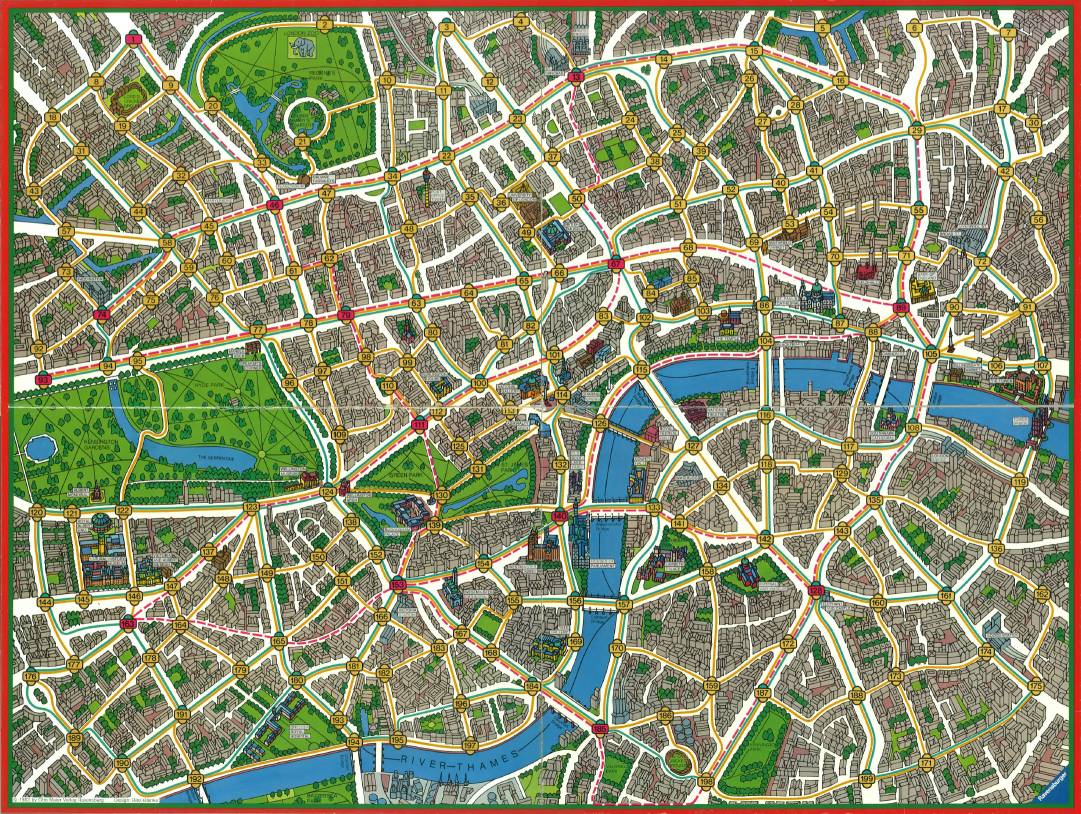
\includegraphics[scale=0.3]{img/einleitung/Spielplan.png}
        \end{center}
        Neben dem Spielplan ist die jeweils aktuelle Fahrtentafel von Mister X zu sehen - also eine Anzeige seiner Züge bzw. der jeweils dafür verbrauchten Tickets.
        Die Aufteilung soll wie im Beispielprogramm 3 Spalten und eine Nummerierung von 1 bis 24 vorsehen und außerdem kenntlich machen, welche der Züge verdeckt und welche die \textit{Zeigezüge} von Mister X sind.
        Ob Ihr hier ein komplettes Bild der Fahrtentafel ladet und nutzt oder eine eigene Darstellungsform wählt, ist Euch freigestellt.
        Es müssen hier nur die verbrauchten Tickets sichtbar sein, die Zugstationen sind ja eh geheim.
        \newline
        \newline
        Weiterhin soll die Oberfläche den am Zug befindlichen Spieler (bzw. Mister X) und seine noch vorhandenen Tickets anzeigen, wobei jeweils das entsprechende Bild des Tickets sowie als Textausgabe die vorhandene Anzahl darzustellen sind.
        (Im Archiv der Ticketbilder findet sich auch eines für eine mögliche Startposition.
        Wer möchte, darf auch diese irgendwie auf der Oberfläche mit darstellen)

    \section{Steuerung}
        Zu Beginn eines neuen Spiels wird der Spieler gefragt, ob er Mister X und/oder die Detektive steuern möchte (andernfalls macht dies jeweils die KI) und wie viele Detektive (3, 4 oder 5) mitspielen sollen.
        Danach sind immer abwechselnd Mister X und die Detektive in der o.g. Reihenfolge am Zug.
        Die Detektive werden immer komplett entweder von der KI oder vom Spieler gesteuert.
        \newline
        \newline
        Der Spieler kann mit der Maus auf eine beliebige Stelle des Spielplans klicken.
        Es soll dann die Station von 1 bis 199 bestimmt werden, die den geringsten Abstand zu der Klickposition hat (gemeint ist hier die Luftlinie, also der euklidische Abstand --> Satz des Pythagoras).
        Allerdings soll hier ein Maximalabstand definiert werden, so daß nur Klicks, die eine Station auch grob treffen (und nicht irgendwo im Park liegen), als zu dieser Station gehörig gezählt werden.
        Falls diese Station zu derjenigen \textit{benachbart} ist, an der sich der aktuelle Spieler gerade befindet (also mindestens ein Verkehrsmittel dahin führt) und dieser Spieler auch noch ein passendes Ticket hat, wird er auf die benachbarte Station bewegt und das passende Ticket wird aus seinem Vorrat entfernt bzw. geht an Mister X.
        Falls es mehrere mögliche Verkehrsmittel für die Strecke gibt, soll der Spieler (z.B. über ein Popupmenü wie im Beispielprogramm) entscheiden können, welches davon er nehmen möchte.
        \newline
        \newline
        Falls der Spieler auch Mister X steuert, ist das Verhalten hier dasselbe, nur daß verbrauchte Tickets einfach aus seinem Vorrat verschwinden.
        Die Fahrtentafel wird parallel zu seinen Zügen mit Tickets gefüllt.
        \newline
        \newline
        Kann ein Detektiv nicht mehr ziehen, weil er keine Tickets mehr hat, die von seiner aktuellen Station wegführen, wird er im Ablauf aller Detektive ausgelassen.
        Kann kein Detektiv mehr ziehen, hat Mister X gewonnen.
        \newline
        \newline
        Wo sich welche Station befindet und welche Verkehrsmittel dort wohin genommen werden können, ist in der netz.json hinterlegt.
        Diese beinhaltet
        \begin{itemize}
            \item die Nummer der Station
            \item die Pixelposition auf dem Spielplan (0/0 ist oben links, 1/1 ist unten rechts)
            \item die per U-Bahn zu erreichenden Stationen aufsteigend
            \item die per Bus zu erreichenden Stationen aufsteigend
            \item die per Taxi zu erreichenden Stationen aufsteigend
            \item die per Boot zu erreichenden Stationen aufsteigend.
        \end{itemize}
        Hilfe zum Parsen einer JSON-Datei findet sich unten.
        \newline
        \newline
        Es bietet sich an, alle 199 Stationen in einem Array zu verwalten.
        Die Verbindungen zu anderen Stationen eines Typs lassen sich jeweils gut in einer Menge ablegen.

    \section{KI}
        Sowohl die Detektive als auch Mister X können optional auch von einer KI gesteuert werden.
        Auch die Steuerung von beiden \textit{Parteien} in einem Spiel durch die KI soll möglich sein.
        Es wird von der KI dann jeweils der optimale nächste Zug bestimmt und die Spieler bzw. Mister X bewegen sich entsprechend zu den neuen Positionen.
        Natürlich sollen auch hier nur Züge auf \textit{benachbarte} Stationen möglich sein und es können nur Verkehrsmittel verwendet werden, für die noch ein Ticket vorliegt (die Spielregeln sind also einzuhalten). 
        \newline
        \newline
        Zur Bestimmung eines optimalen Spielerzuges soll folgendes Vorgehen umgesetzt werden (wodurch Spielsituationen vergleichbar und nachvollziehbar werden): 
        \begin{itemize}
            \item es werden folgende verschiedene Taktiken alle nacheinander durchgespielt (Achtung: Die Beispiele mit --> beziehen sich hier immer nur auf genau EINE Taktik. In Wirklichkeit sollen ALLE durchprobiert und die bestbewertetste genommen werden!)
                \begin{itemize}
                    \item bewege Dich auf eine mögliche Zielposition (s.u., auf dem Bild rechts hellgrün eingekreist. Mister X ist also von der letzten Zeigeposition bei 116 aus 1x Taxi gefahren). Gibt es mehrere erreichbare, wähle davon die mit der kleinsten Stationsnummer --> der blaue Detektiv würde sich demnach zu Station 118 begeben
                    \item bewege Dich auf eine direkt benachbarte U-Bahn-Station (um schnell zu anderen Standorten zu kommen). Gibt es mehrere erreichbare freie, wähle davon die mit der kleinsten Stationsnummer --> der gelbe Detektiv würde sich demnach zu Station 185 begeben
                    \item bewege Dich in Richtung auf die letzte Zeigeposition von Mister X (s.u.). Benutze dafür den kürzesten (derzeit) freien Weg --> der rote Detektiv würde sich demnach zu Station 70 (und folgend zu 87, 86, 116) begeben, weil dies die erste auf dem kürzesten Weg ist und sie zudem eine kleinere Nummer als die 89 hat (s.u.)
                    \item bewege Dich auf diejenige direkt benachbarte freie Position mit der kleinsten Stationsnummer (quasi als Fallback, wenn nichts anderes funktioniert)
                \end{itemize}
            \item nach jedem versuchten Zug wird die neue Spielsituation (Spieler zieht auf Station x) anhand der folgend beschriebenen Bewertungsfunktion eingeschätzt. Der bestbewertete Zug wird umgesetzt (bei mehreren mit identischer Bewertung wird die Station mit der kleineren Nummer genommen). Die Bewertungsfunktion setzt sich aus diesen Einzelwerten und Gewichten zusammen, die aufaddiert werden. Ein größerer Wert ist besser:
                \begin{itemize}
                    \item wie viele mögliche Zielpositionen sind für alle Detektive im nächsten Zug erreichbar [genauer formuliert am 29.10.: wie viele der möglichen Zielpositionen sind im nächsten Zug von jeweils mindestens einem Detektiv erreichbar] geteilt durch die Gesamtzahl aller möglichen Zielpositionen (für die noch nicht gezogenen Detektive sollen hierbei noch ihre alten Stationen berücksichtigt werden)
                    \newline
                    \textbf{Gewichtung:} Anzahl erreichbarer Zielpositionen durch Gesamtzahl der Zielpositionen * 10
                    \newline
                    --> nachdem der blaue Detektiv auf Station 118 gezogen ist, blieben noch 3 Zielpositionen übrig (104, 117, 127), die aber alle nicht erreicht werden können
                    \newline
                    --> 0 / 3 * 10 = 0
                    \item wie weit ist die \textit{mittlere mögliche Zielposition} (s.u.) entfernt (damit die Detektive, die weiter von Mister X weg sind, sich grob in seine Richtung bewegen und nicht dumm in der Gegend rumlaufen)
                    \newline
                    \textbf{Gewichtung:} wenn 10 Stationen oder mehr weg = 0, ansonsten (10 - Anzahl Stationen auf dem kürzesten Weg zur \textit{mittleren möglichen Zielposition})
                    \newline
                    --> nachdem der blaue Detektiv auf Station 118 gezogen ist, blieben noch 3 Zielpositionen übrig (104, 117, 127). Deren Koordinaten sind 765/341, 848/447 und 693/447, gemittelt also 769/412. Daran am dichtesten liegt Station 116, die genau 1 Station von 118 entfernt ist
                    \newline
                    --> (10 - 1) = 9
                    \item wie viele Stationen sind von der aktuellen Position aus mit den vorhandenen Tickets in einem Zug erreichbar
                    Gewichtung: Anzahl Stationen geteilt durch 13 (da dies bei Station 67 die meisten unterschiedlichen erreichbaren Stationen sind) * 4
                    \newline
                    --> angenommen, der blaue Detektiv hat noch 3 U-Bahn-, 4 Bus- und 3 Taxitickets, dann kann er von Station 118 aus 4 andere Stationen (alle per Taxi) erreichen
                    \newline
                    --> 4 / 13 * 4 = 1,23
                    \item was ist die geringste Ticketanzahl für ein Verkehrsmittel (hat man für eines gar kein Ticket mehr, schränkt das die Mobilität deutlich ein)
                    \newline
                    \textbf{Gewichtung:} Wenn es noch mehr als 2 Tickets sind, ist die Bewertung 3, ansonsten Anzahl der Tickets.
                    \newline
                    --> die geringste Zahl von Tickets beim blauen Detektiv (s.o.) ist 3
                    \newline
                    --> = 3
                    \newline
                    --> die gesamte Bewertung wäre also 0 + 9 + 1,23 + 3 = 13,23
                \end{itemize}
            \item zur besseren Nachvollziehbarkeit der KI-Schritte sollen die Einzelwerte der Bewertungsfunktion zusammengefasst und im Log (s.u.) ausgegeben werden können
        \end{itemize}
        Alle Spieler sind dabei nacheinander mit dem genannten Vorgehen an der Reihe.
        Es gibt somit keine \textit{Gruppenabsprachen} der Detektive o.ä. Sollte tatsächlich einmal der Fall eintreten, daß alle Nachbarstationen besetzt sind, bewegt sich ein Detektiv in diesem Zug nicht, gibt dafür aber natürlich auch kein Ticket ab.
        Ansonsten muß ein Detektiv (und auch Mister X) aber ziehen, wenn dies möglich ist.
        \newline
        \newline
        Immer dann, wenn bei einer Taktik mehrere Verkehrsmittel möglich sind, soll dasjenige genommen werden, von wem noch am meisten vorhanden sind (siehe Bewertungsfunktion).
        Gibt es davon gleich viele und mehrere sind für den Zug möglich, sollen diese in der Reihenfolge Taxi -> Bus -> U-Bahn (-> Boot) benutzt werden, also von \textit{wertlos} zu \textit{wertvoll}. 
        \newline
        \newline
        Eine \textbf{mögliche Zielposition} ist eine Station, an der sich Mister X gerade befinden könnte.
        Dies hängt offenkundig davon ab, wo er sich zuletzt gezeigt hat, wie viele Züge seitdem vergangen sind, wo die Detektive sich befinden und welche Tickets er benutzt hat.
        Diese Menge von Stationen soll von Euch für die KI berechnet und genutzt werden. Die mittlere mögliche Zielposition ergibt sich aus einer Mittelung der Koordinaten in X und Y (aus der Netz.json) aller möglichen Zielpositionen und anschließender Bestimmung derjenigen Station, die sich am dichtesten (Luftlinie) an dieser mittleren Koordinate befindet. 
        \newline
        \newline
        Bei einer \textbf{Bewegung in Richtung auf die letzte Zeigeposition} von Mister X soll im Netz der Weg mit den wenigsten Zwischenstationen gesucht werden.
        Hierbei ist zu berücksichtigen, über welche Tickets ein Spieler noch verfügt. Hat er beispielsweise keine Bustickets mehr, darf die Route auch keine Busstrecken beinhalten. Dies kann im Extremfall heißen, daß kein Weg möglich ist.
        Ebenso dürfen keine Knoten im Weg vorkommen, die (derzeit) von Detektiven belegt sind. Falls mehrere Wege gleich kurz sind (also über dieselbe Anzahl an Zwischenstationen gehen), soll davon derjenige benutzt werden, der im ersten Schritt zur kleineren Stationsnummer führt. 
        \newline
        \newline
        Die KI für Mister X arbeitet identisch zu der der Spieler-KI, nur daß eine andere Taktik und andere Bewertungen berücksichtigt werden sollen.
        Teilweise können hier aber Funktionen der Spieler-KI wiederverwendet werden!
        \begin{itemize}
            \item \textbf{Taktik} von Mister X
                \begin{itemize}
                    \item bewege Dich auf eine Station, die möglichst wenige Spieler im nächsten Zug erreichen können. Hierfür werden bei Mister X einfach alle erreichbaren Stationen durchgetestet
                \end{itemize}
            \item \textbf{Bewertungsfunktion} von Mister X
                \begin{itemize}
                    \item wie viele Detektive können die Position von Mister X im nächsten Zug erreichen
                    Gewichtung: (Gesamtzahl Detektive - Anzahl Detektive, die Mister X erreichen können) * 10
                    Hierbei ist zu berücksichtigen, welche Tickets die Detektive noch haben (dies weiß Mister X im echten Spiel ja auch). Ggf. kann also ein Detektiv Mister X auf der direkten Nachbarstation nicht erreichen, weil ihm das passende Ticket fehlt...
                    \item wie viele Stationen kann Mister X von der aktuellen Position aus mit den vorhandenen Tickets in einem Zug erreichen, auf denen kein Detektiv steht
                    Gewichtung: Anzahl Stationen geteilt durch 13 (da dies bei Station 67 die meisten unterschiedlichen erreichbaren Stationen sind) * 4
                    \item was ist die geringste Ticketanzahl für ein Verkehrsmittel (hat man für eines gar kein Ticket mehr, schränkt das die Mobilität deutlich ein)
                    Gewichtung: Wenn es noch mehr als 2 Tickets sind, ist die Bewertung 3, ansonsten Anzahl der Tickets
                \end{itemize}
            \item auch hier sollen die Schritte mit in die Logdatei geschrieben werden (s.u.)
        \end{itemize}
        Mit dem beschriebenen KI-Vorgehen ist es leicht möglich, weitere Taktiken zu ergänzen, bestehende zu entfernen oder andere Gewichtungen der Bewertung vorzunehmen.
        Sie stellt somit eine brauchbare und in der KI verbreitete Mittellösung zwischen \textit{alle möglichen Kombinationen von Zügen in einen Baum stecken und durchlaufen für x Ebenen} und dem simplen \textit{wenn Zug A möglich ist, mache den, sonst wenn B möglich ist mache ...} dar. 

    \section{Log}
        Zur Nachvollziehbarkeit soll pro Spiel eine Logdatei (als einfache Textdatei mit der Endung *.log) geschrieben werden (es gibt genau eine, zu Beginn eines neuen Spiels wird diese also gelöscht bzw. überschrieben).
        Sie soll folgende Informationen exakt im angegebenen Format beinhalten:

        \begin{itemize}
            \item die Anzahl der Detektive (ganze Zahl)
            \item ob MisterX von der KI gesteuert wird (true oder false)
            \item ob die Detektive von der KI gesteuert werden (true oder false)
            \item die Startposition von MisterX
            \item die Startpositionen aller teilnehmenden Detektive
            \newline
            --> alle Werte bis hier werden kommasepariert in einer Zeile abgelegt
            \item alle Züge der Spieler bzw. von Mister X jeweils kommasepariert in einer Zeile, wie folgt:
                \begin{itemize}
                    \item welcher Spieler zieht (ganze Zahl ab 1 für die Detektive, 0 für MisterX)
                    \item bisherige Station
                    \item neue Station
                    \item restliche Tickets für U-Bahn, Bus, Taxi, Boot (bei den Detektiven stets 0)
                    \item welche der Taktiken (ab 1 in der o.g. Reihenfolge) wurde gewählt (bei einem menschlichen Spielzug = 0)
                    \item wie sieht die Bewertung (siehe oben) dazu aus (bei einem menschlichen Spielzug = 0.0)
                    \newline
                    --> hierbei soll zur besseren Lesbarkeit ein Dezimalpunkt verwendet werden
                \end{itemize}
            \item wer das Spiel gewonnen hat (0 für Mister X, 1 für die Detektive)
        \end{itemize}
        Hier findet sich ein Beispiellog für ein relativ kurzes Spiel zum Vergleich (Init + 2 KI-Züge von Mister X und dazwischen ein menschlicher Zug von 3 Detektiven). 

    \section{Spielstand}\label{spielstand}
        Der aktuelle Spielstand soll jederzeit in einer vom Benutzer wählbaren Datei gespeichert und aus einer frei wählbaren Datei wieder geladen werden können. Seht hier bitte ggf. Rückfragen an den Nutzer vor, damit keine Spielstände ungewollt überschrieben oder gelöscht werden.
        \newline
        \newline
        Eine Spielstandsdatei (ebenfalls eine JSON-Datei) hat folgende Einträge:
        \begin{itemize}
            \item MisterX
                \begin{itemize}
                    \item ob er von der KI gesteuert wird (true oder false)
                    \item die möglichen Zielpositionen 
                    \item die letzte Zeigeposition (oder 0, wenn es noch keine gab)
                    \item die aktuelle Station
                    \item alle restlichen Tickets von Mister X (ganze Zahlen für U-Bahn, Bus, Taxi, Boot)
                    \item die belegten Einträge der Fahrtentafel (Ordinalwerte der verbrauchten Tickets ab 0 in der Reihenfolge U-Bahn, Bus, Taxi, Boot)
                \end{itemize}
            \item Detektive
                \begin{itemize}
                    \item die Anzahl der Detektive (ganze Zahl)
                    \item ob sie von der KI gesteuert werden (true oder false)
                    \item für jeden Detektiv
                    \begin{itemize}
                        \item die aktuelle Station
                        \item alle restlichen Tickets (ganze Zahlen für U-Bahn, Bus, Taxi)
                    \end{itemize}
                \end{itemize}
            \item wer am Zug ist (0 = Mister X, Detektive ab 1)
            \item die wievielte Runde es ist (beginnend bei 1)
            \item ob das Spiel schon gewonnen wurde (true oder false)
        \end{itemize}
        Hier findet sich ein Beispielspielstand für ein relativ kurzes Spiel zum Vergleich (passend zum obigen Log).
        Sollten beim Speichern Fehler auftreten, wird der Nutzer darüber mit einer Meldung informiert.
        Sollten beim Laden Fehler auftreten, soll der Nutzer ebenfalls informiert und der bisherige Zustand des Spiels weiterverwendet werden. Nach einem erfolgreichen Laden wird das bisherige Log gelöscht und ein neues angelegt, als hätte gerade ein neues Spiel begonnen.
        Als Startpositionen werden die aktuellen Positionen genommen.

    \section{Zwischenstand}
        Bei der Abnahme des Zwischenstands müssen die Vorgaben erfüllt werden:
        \begin{itemize}
            \item \textbf{GUI}
                \begin{itemize}
                    \item In einer FXML-Datei müssen alle Bedienelemente enthalten sein, die für eine Bedienung des Programms notwendig sind.
                    \item Es muss erkennbar sein, wie angezeigt wird, welche Fahrkarten ein Spieler noch zur Verfügung hat.
                    \item Eine Fahrtentafel mit Kennzeichnung der Züge, bei denen Mister X sich zeigt, muss sichtbar sein.
                    \item Nach Programmstart muss das Spielfeld sichtbar sein und sich bei Änderung der Fenstergröße gleichermaßen ändern.
                    \item Es muss eine Station angewählt werden können, was zu einer sichtbaren Reaktion führt (es genügt die Markierung mit einem Kreis). Die Markierung muss bei Änderung der Fenstergröße auf der Station bleiben.
                \end{itemize}
            \item \textbf{Datenstrukturen} müssen erkennen lassen
                \begin{itemize}
                    \item wie und wo die Spieler definiert werden
                    \item wie die Netzstruktur abgelegt wird
                    \item welche Struktur einen Spielstand abbildet
                    \item wie/wo die verschiedenen Taktiken eines Spielers eingesetzt werden (welche Methoden welcher Klassen)
                \end{itemize}
            \item \textbf{Tests} dürfen noch fehlschlagen, müssen aber vorhanden und kompilierbar sein und natürlich die korrekten Erwartungswerte enthalten. Mehrere Konstruktoren sind zu erstellen, um eine Spielsituation für einen Test erstellen zu können. Mindestens folgende Testfälle müssen abgedeckt werden:
                \begin{itemize}
                    \item auf welchen Positionen kann Mister X im aktuellen Zug stehen (mögliche Zielpositionen)
                    \item wurde Mister X gefangen
                    \item jeweils zwei sinnvolle Tests für jede der 3 erstgenannten Taktiken; einer davon prüft, ob aus mehreren möglichen Stationen die kleinere gewählt wird
                    \item ein Test für die viertgenannte Taktik
                    \item ein Test für jede der 4 Einzelbewertungen einer Situation
                    \item die Wahl der bestbewerteten Taktik
                \end{itemize}
        \end{itemize}